\documentclass[handout]{beamer}


\usetheme{default}
\usepackage{subfigure}
\usepackage{amsmath}
\usepackage{Sweave}
\usepackage{graphicx}
\usepackage{color}
\usepackage{amsfonts}
\usepackage{amssymb}
\usepackage{multicol}
\usepackage[all]{xy}
\usepackage{bm}


\author{Patrick Lam}
\title{Model Checking}
\date{}
%\date{December 1, 2008}

\begin{document}

\newcommand{\red}{\textcolor{red}}
\newcommand{\blue}{\textcolor{blue}}
\newcommand{\purple}{\textcolor{purple}}

\frame{\titlepage}

\begin{frame}
\frametitle{Outline}
\tableofcontents
\end{frame}

\section{Posterior Predictive Distribution}

\begin{frame}
\frametitle{Outline}
\tableofcontents[currentsection]
\end{frame}

\begin{frame}
\frametitle{Prediction}
\pause
Once we have a model and generated draws from our \blue{posterior}
distribution, we may want to predict future data points.  \\
\pause
\bigskip
We may want to make predictions in order to:
\pause
\begin{enumerate}
\item Predict how a system would behave in the future (substantive implications)
\pause
\item Assess model accuracy (modeling implications)
\end{enumerate}
\pause
\bigskip
Through simulation, we can get a \textbf{posterior predictive distribution}.
\end{frame}

\begin{frame}
\frametitle{Posterior Predictive Distribution}
\pause
Predicted distribution of some future data point(s) $y^{\mathrm{rep}}$ after
having seen the data $y$.
\pause
\begin{eqnarray*}
p(y^{\mathrm{rep}} | y) &=& \int p(y^{\mathrm{rep}}, \theta | y) d\theta \\
&=& \int p(y^{\mathrm{rep}} | \theta, y) \textcolor{blue}{p(\theta | y)} d\theta
\end{eqnarray*}
\pause
If we assume $y \bot y^{\mathrm{rep}} | \theta$, then
\pause
\begin{eqnarray*}
p(y^{\mathrm{rep}} | y) &=&  \int p(y^{\mathrm{rep}} | y) \textcolor{blue}{p(\theta | y)} d\theta
\end{eqnarray*}
\pause
If $y$ is a vector of $n$ observations, then $y^{\mathrm{rep}}$ is
also a vector of length $n$ with covariates set at the observed (model
checking) or hypothetical values (prediction) \pause and
$p(y^{\mathrm{rep}} | y)$ can be thought of as an $n$-variate distribution.
\end{frame}

\begin{frame}[fragile]
We can simulate the \textcolor{blue}{posterior} predictive distribution.
\pause
\bigskip
\begin{enumerate}
\item Sample $m$ values of $\theta$ from our \textcolor{blue}{posterior}.
\pause
\item For each \textcolor{blue}{posterior} draw, sample a value (vector) of
$y^{\mathrm{rep}}$ from our likelihood $p(y^{\mathrm{rep}} | \theta)$.
\end{enumerate}
\bigskip
\pause
The $m$ values (vectors) of $y^{\mathrm{rep}}$ represent draws from
the \blue{posterior} predictive distribution $p(y^{\mathrm{rep}} | y)$.\\
\pause
\bigskip
We can use the posterior predictive distribution to predict the future
or assess model accuracy with posterior predictive checks.
\end{frame}

\section{Posterior Predictive Checks}

\begin{frame}
\frametitle{Outline}
\tableofcontents[currentsection]
\end{frame}

\begin{frame}
Much of what we have done so far is based on
a model that we specify, which may or may not be accurate. \\
\bigskip
\pause
Specifically, we make many assumptions with our model which may or may
not be accurate (for example, independence across observations). \\
\bigskip
\pause
We can attempt to check specific model assumptions with \textbf{posterior predictive checks}.
\end{frame}

\begin{frame}
\frametitle{Posterior Predictive Checks}
\pause
To conduct a posterior predictive check, do the following:
\medskip
\pause
\begin{enumerate}
\item Come up with a test statistic $T$ that has power to diagnose
violations of whatever assumption you are testing. 
\medskip
\pause
\item Calculate $T$ for the observed data $y$: \pause $T(y)$
\medskip
\pause
\item Calculate $T$ for each $y^{\mathrm{rep}}$ draw from the
posterior predictive distribution: \pause $T(y^{\mathrm{rep}} | y)$
\medskip
\pause
\item Calculate the fraction of times $T(y^{\mathrm{rep}} | y) >
T(y)$.  \pause  This is an estimate of the \textit{posterior
predictive $p$-value}. 
\end{enumerate}
\end{frame}

\begin{frame}
The idea is that if our data violates one of our model assumptions,
then our observed test statistic $T(y)$ should be significantly
different than our model predicted test statistics $T(y^{\mathrm{rep}} | y)$.\\
\bigskip
\pause
If our posterior predictive $p$-value is close to 0 or 1 (say 0.05 or
0.95), then it suggests that our observed data has an extreme test
statistic and that something in our model may be inadequate.
\end{frame}

\begin{frame}
\frametitle{Possible Problems with Posterior Predictive Checks}
\pause
\begin{itemize}
\item Choice of test statistic is very important.
\pause
\begin{itemize}
\item Test statistic must be meaningful and pertinent to the
assumption you want to test.
\pause
\item Test statistics often have low power (inability to find problems
when problems exist)
\pause
\item Test statistics should be not based on aspects of the data that
are being explicit modeled (for example, the mean of $y$ in a linear model).
\end{itemize}
\pause
\medskip
\item If the model passes posterior predictive check, it does not
necessarily mean there are no problems with the model.
\begin{itemize}
\pause
\item Test statistic may have low power.
\pause
\item May be testing the wrong assumption.
\end{itemize}
\pause
\medskip
\item It is not always clear how to correct the incorrect model assumptions.
\end{itemize}
\end{frame}

\subsection{An Example}

\begin{frame}
\frametitle{Outline}
\tableofcontents[currentsubsection]
\end{frame}

\begin{frame}[fragile]
\frametitle{Running Example}
\pause
Time-series cross-sectional dataset on civil war onset from Fearon and Laitin.
\pause
\tiny
\medskip
\begin{Schunk}
\begin{Sinput}
> data <- read.table("FLdata.txt")
\end{Sinput}
\end{Schunk}
\normalsize
\pause
\bigskip
Dependent variable: binary variable on civil war onset\\
\pause
\bigskip
Independent variables: the normal set of independent variables
predicting civil wars \\
\pause
\bigskip
Model: Bayesian logistic regression with binomial likelihood and
multivariate Normal priors (using {\tt MCMCpack})
\pause
\tiny
\medskip
\begin{Schunk}
\begin{Sinput}
> library(MCMCpack)
> posterior <- MCMClogit(new.onset ~ warl + gdpenl + lpopl1 + lmtnest + 
+     ncontig + Oil + nwstate + instab + polity2l + ethfrac + relfrac, 
+     data = data, tune = 0.6, burnin = 1000, mcmc = 5000)
\end{Sinput}
\begin{Soutput}
@@@@@@@@@@@@@@@@@@@@@@@@@@@@@@@@@@@@@@@@@@@@@@@@@@@@@@@@
The Metropolis acceptance rate for beta was 0.32250
@@@@@@@@@@@@@@@@@@@@@@@@@@@@@@@@@@@@@@@@@@@@@@@@@@@@@@@@
\end{Soutput}
\end{Schunk}
\normalsize
\end{frame}

\begin{frame}[fragile]
\frametitle{Posterior Predictive Distribution}
\pause
\begin{enumerate}
\item Create model matrix of covariates $X$.
\tiny 
\medskip
\pause
\begin{Schunk}
\begin{Sinput}
> X <- cbind(1, data[, c("warl", "gdpenl", "lpopl1", "lmtnest", 
+     "ncontig", "Oil", "nwstate", "instab", "polity2l", "ethfrac", 
+     "relfrac")])
\end{Sinput}
\end{Schunk}
\pause
\normalsize
\medskip
\item Get linear predictors by multiplying $X$ and our $m$ draws from
the posterior.
\tiny 
\medskip
\pause
\begin{Schunk}
\begin{Sinput}
> Xb <- as.matrix(X) %*% t(posterior)
\end{Sinput}
\end{Schunk}
\pause
\normalsize
\medskip
\item Convert linear predictors into probabilities with the inverse logit function.
\tiny 
\medskip
\pause
\begin{Schunk}
\begin{Sinput}
> probs <- 1/(1 + exp(-Xb))
\end{Sinput}
\end{Schunk}
\pause
\normalsize
\medskip
\item Draw $m$ samples of $y^{\mathrm{rep}}$ from the binomial likelihood.
\tiny 
\medskip
\pause
\begin{Schunk}
\begin{Sinput}
> n <- nrow(X)
> m <- nrow(posterior)
> y.rep <- matrix(NA, nrow = n, ncol = m)
> for (i in 1:m) {
+     y.rep[, i] <- rbinom(n, size = 1, prob = probs)
+ }
\end{Sinput}
\end{Schunk}
\pause
\normalsize
\end{enumerate}
The resulting posterior predictive distribution is an $n \times m$
matrix.
\end{frame}

\begin{frame}
\frametitle{A Bad Test Statistic}
\pause
Let $T$ = the fraction of y's that take on the value of 1 \\
\bigskip
\pause
What's wrong with this test statistic?
\pause
\medskip
\begin{itemize}
\item Unclear what assumption are we testing.
\pause
\item The fraction of 1s is explicitly being modeled in the logit model.
\pause
\begin{itemize}
\item The test will never show anything is wrong regardless of how bad
our model is.
\end{itemize}
\end{itemize}
\end{frame}

\begin{frame}
\frametitle{A Better Test Statistic}
\pause
Assumption: No clustering within years\\
\pause
\bigskip
Test Statistic: $T$ = the variance of the number of 1s in each year
\end{frame}

\begin{frame}[fragile]
\begin{enumerate}
\item Come up with a test statistic $T$ that has power to diagnose
violations of whatever assumption you are testing: \pause  $T$ = the variance of the number of 1s in each year
\medskip
\pause
\item Calculate $T$ for the observed data $y$: \pause $T(y)$
\medskip
\pause
\tiny
\begin{Schunk}
\begin{Sinput}
> emp.year.sum <- c()
> for (i in 1:length(unique(data$year))) {
+     emp.year.sum[i] <- sum(data$new.onset[which(data$year == 
+         unique(data$year)[i])])
+ }
> T.y <- var(emp.year.sum)
\end{Sinput}
\end{Schunk}
\pause
\medskip
\normalsize 
\item Calculate $T$ for each $y^{\mathrm{rep}}$ draw from the
posterior predictive distribution: \pause $T(y^{\mathrm{rep}} | y)$
\medskip
\pause
\tiny
\begin{Schunk}
\begin{Sinput}
> year.sum <- matrix(NA, nrow = length(unique(data$year)), ncol = ncol(y.rep))
> for (i in 1:length(unique(data$year))) {
+     year.sum[i, ] <- apply(y.rep[which(data$year == unique(data$year)[i]), 
+         ], 2, sum)
+ }
> T.y.rep <- apply(year.sum, 2, var)
\end{Sinput}
\end{Schunk}
\end{enumerate}
\normalsize 
\end{frame}

\begin{frame}[fragile]
\begin{enumerate}
\item[4.] Calculate the fraction of times $T(y^{\mathrm{rep}} | y) >
T(y)$.  \pause  This is an estimate of the \textit{posterior
predictive $p$-value}. 
\medskip
\pause
\tiny
\begin{Schunk}
\begin{Sinput}
> mean(T.y.rep > T.y)
\end{Sinput}
\begin{Soutput}
[1] 0.107
\end{Soutput}
\end{Schunk}
\end{enumerate}
\begin{figure}[!htp]
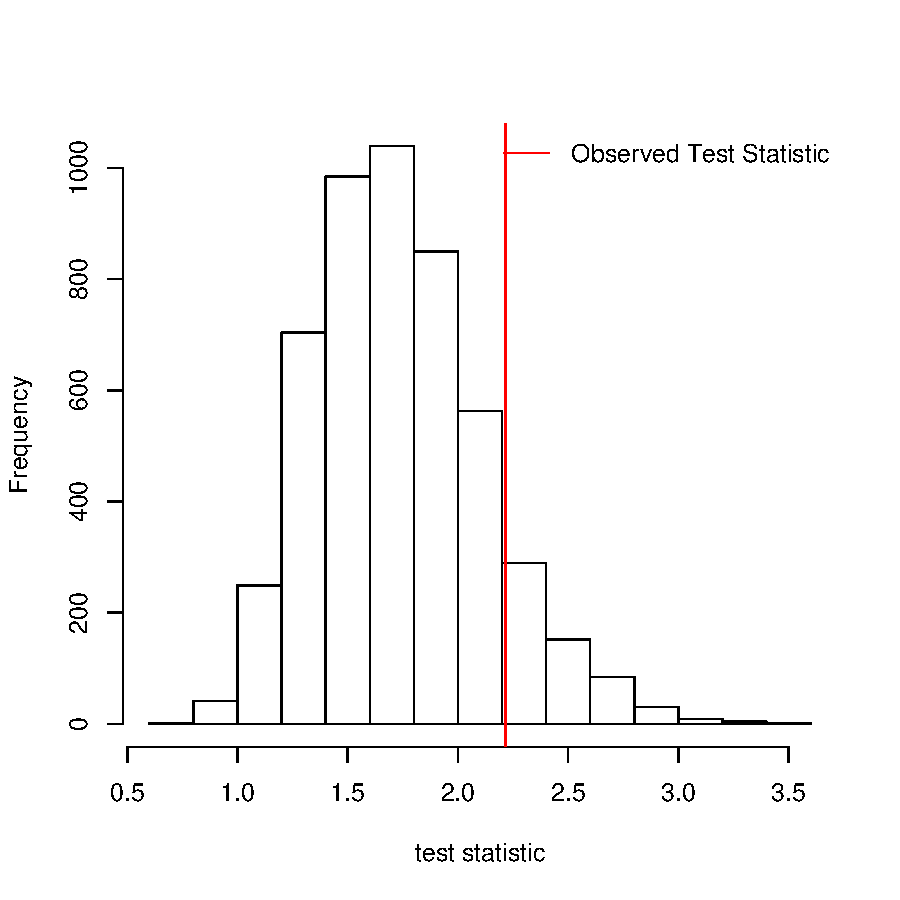
\includegraphics[width = 1.5in, height=1.5in]{modelcheck-yearhist.pdf}
\end{figure}
\normalsize
\pause
Does this mean our assumption is correct?  \pause Not necessarily (low
power?)
\end{frame}
\end{document}
